\documentclass[11pt]{article}
\usepackage{hyperref} 
\usepackage{amsmath, amsfonts, amssymb}
\usepackage{graphicx}
\usepackage{float}
\usepackage[margin=1in]{geometry}
\usepackage{cancel}

\parindent0px

\emergencystretch=0pt
\pretolerance=150
\tolerance=10000
\hbadness=10000
\hfuzz=0pt

\title{Introduction to Linear Algebra Notes}
\author{Nathan Ueda}
\date{\today} 

\begin{document}
\maketitle 
\pagebreak
\tableofcontents 
\pagebreak

\section{Vectors and Matrices}
\subsection{Vectors and Linear Combinations}

\textbf{Vector Length:} For a vector $ \boldsymbol{v} \in \mathbb{R}^n $, its length is:

\[ \|\boldsymbol{v}\|= \sqrt{v_1^2 + \cdots + v_n^2} \]

In words, the length of a vector is the square root of the sum of the squared components. \\

Given two vectors in $\mathbb{R}^2\ \boldsymbol{v}, \boldsymbol{w}$ with their tail starting 
from the origin
\begin{itemize}
    \item If they lie on the same line, the vectors are \textit{linearly dependent}.
    \item If they do not lie on the same line, the vectors are \textit{linearly independent}.
\end{itemize}
Therefore, the combinations $ c\boldsymbol{v} + d\boldsymbol{w} $ fill the $x-y$ plane unless 
$\boldsymbol{v}$ is in line with $\boldsymbol{w}$. \\

To fill $m$-dimensional space, we need $m$ independent vectors, with each vector having $m$
components.

\subsection{Lengths and Angles from Dot Products}

\textbf{Dot Product:} For two vectors $\boldsymbol{v}, \boldsymbol{w} \in \mathbb{R}^n$, their
dot product is:

\[ \boldsymbol{v} \cdot \boldsymbol{w} = v_1 w_1 + \cdots + v_n w_n \]

The dot product of two vectors tells us what amount of one vector goes in the direction of
another. It tells us how much these vectors are working together.

\begin{itemize}
    \item $ \boldsymbol{v} \cdot \boldsymbol{w} > 0 $: The vectors point in somewhat similar 
    directions. In other words, the angle between the two vectors is less than 90 degrees.
    \item $ \boldsymbol{v} \cdot \boldsymbol{w} = 0 $: The vectors are perpendicular. In other 
    words, the angle between the two vectors is 90 degrees.
    \item $ \boldsymbol{v} \cdot \boldsymbol{w} < 0 $: The vectors point in somewhat opposing 
    directions. In other words, the angle between the two vectors is greater than 90 degrees.
\end{itemize}

Dot Product Rules (for two vectors, $\boldsymbol{v}, \boldsymbol{w}$):
\begin{itemize}
    \item $ \boldsymbol{v} \cdot \boldsymbol{w} = \boldsymbol{w} \cdot \boldsymbol{v} $
    \item $ \boldsymbol{u} \cdot (\boldsymbol{v} + \boldsymbol{w}) = \boldsymbol{u} \cdot 
    \boldsymbol{v} + \boldsymbol{u} \cdot \boldsymbol{w} $
    \item $ (c\boldsymbol{v}) \cdot \boldsymbol{w} = c(\boldsymbol{v} \cdot \boldsymbol{w}) $
\end{itemize}

\textbf{Cosine Formula:} If $\boldsymbol{v}$ and $\boldsymbol{w}$ are nonzero vectors, then:
\[ \cos \theta = \frac{\boldsymbol{v} \cdot \boldsymbol{w}}{\|\boldsymbol{v}\| \|\boldsymbol{w}
\|}\]

\textbf{Unit Vectors:} A vector is a unit vector if its length is 1. \\
For a vector $\boldsymbol{u} \in \mathbb{R}^n$:

\[ \|\boldsymbol{u}\| = 1\]

For any vector $\boldsymbol{v} \in \mathbb{R}^n$, as long as $\boldsymbol{v} \ne 0$, dividing 
$\boldsymbol{v}$ by its length will result in a unit vector. In other words:

\[ \boldsymbol{u} = \frac{\boldsymbol{v}}{\|\boldsymbol{v}\|} \]

\textbf{Cauchy-Schwarz Inequality:} 
\[ | \boldsymbol{v} \cdot \boldsymbol{w} | \le \|\boldsymbol{v}\|  \|\boldsymbol{w}\| \]
In words, the absolute value of the dot product of two vectors is no greater than the product 
of their lengths. \\

\textbf{Triangle Inequality:} 
\[\|\boldsymbol{v} + \boldsymbol{w}\| \le \|\boldsymbol{v}\| + \|\boldsymbol{w}\|\]
In words, the length of any one side (in this case $\|\boldsymbol{v}+\boldsymbol{w}\|$) of a 
triangle is at most the sum of the length of the other triangle sides.

\begin{figure}[H] 
	\centering 
	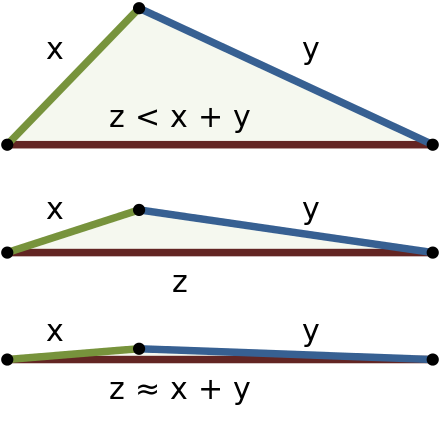
\includegraphics[width=2in]{imgs/triangle_inequality.png}
	\caption{This Squeeze Theorem}
\end{figure}

\subsection{Matrices and Their Column Spaces}

\textbf{Independence:} Columns are independent when each new column is a vector that we don't
already have as a combination of previous columns. The only combindation of columns that produces
$A\boldsymbol{x} = (0,0,0) $ is $ \boldsymbol{x} = (0, 0, 0) $. \\

\textbf{Column Space:} The column space, $\textbf{C}(A)$, contains all vectors 
$A\boldsymbol{x}$. In other words, it contains all combinations of the columns.

The \textbf{span} of the columns of $A$ is the column space. \\

\textbf{Rank}: The number of independent columns of a matrix. This is equivalent to saying the
rank is the number of pivots in a matrix. \\

Rank Rules:
\begin{itemize}
    \item $ \text{rank}(A + B) \le \text{rank}(A) + \text{rank}(B) $
\end{itemize}

\subsection{Matrix Multiplication AB and CR}

To multiply two matrices $AB$, take the dot product of each row of $A$ with each column of $B$. \\ 
The number in row $i$, column $j$ of $AB$ is (row $i$ of $A$) $\cdot$ (column $j$ or $B$). \\

When $A \in \mathbb{R}^{m \times n}$ and $B \in \mathbb{R}^{n \times p}$:
\begin{itemize}
    \item  $AB \in \mathbb{R}^{m \times p}$
    \item $mp$ dot products are needed to carry out the matrix multiplication (one for each 
    entry in the matrix $AB$).
\end{itemize}

Matrix Multiplication Rules:
\begin{itemize}
    \item Associative: $(AB)C$
    \item Distributive: $A(B + C) = AB + BC$
    \item Not Commutative: In general $AB \ne BA$
\end{itemize}

\section{Solving Linear Equations Ax = b}

\subsection{Elimination and Back Substitution}

For a matrix $A \in \mathbb{R}^{n \times n}$, there are three outcomes for 
$A\boldsymbol{x} = \boldsymbol{b}$:

\begin{enumerate}
    \item No solution
    \begin{itemize}
        \item $\boldsymbol{b}$ is not in the column space of $A$
        \item This occurs when the columns of $A$ are dependent and $\boldsymbol{b}$ is not in
        $C(A)$ ($\cancel{32} = \text{any value but 32}$).
        \[\begin{bmatrix}
            2 & 4\\
            4 & 8
            \end{bmatrix} = \begin{bmatrix}
                16 \\
                \cancel{32}
                \end{bmatrix} \]
    \end{itemize}
    \item Exactly 1 solution
    \begin{itemize}
        \item $A$ has independent columns and an inverse matrix $A^{-1}$
    \end{itemize}
    \item Infinitely many solutions
    \begin{itemize}
        \item Columns of $A$ are dependent.
        \item This occurs when the columns of $A$ are dependent and $\boldsymbol{b}$ is in 
        $C(A)$
        \[\begin{bmatrix}
            2 & 4\\
            4 & 8
            \end{bmatrix} = \begin{bmatrix}
                16 \\
                32
                \end{bmatrix} \]
    \end{itemize}
\end{enumerate}

\textbf{Elimination:} A system that allows us to determine if $A\boldsymbol{x} = \boldsymbol{b}
$ has no solution, 1 solution, or infinitely many solutions. The goal of elimination is to
transform $A$ to an upper triangular matrix, $U$. \\ 

Elimination allows us to discover the number of pivots in $A \in \mathbb{R}^{n \times n}$ by 
creating $U$. If there are $n$ pivots in $U$, $U$ has full rank. This implies $A$ has exactly 
one solution. \\

\textbf{Back Substitution}:
If $U$ has full rank, back substituion allows us to find the solution. \\

\subsection{Elimination Matrices and Inverse Matrices}

\textbf{Elimination}

\begin{itemize}
    \item The basic elimination step subtracts a multiple of $\ell_{ij}$ of equation $j$ from
    equation $i$
\end{itemize}

\textbf{Inverse Matrices}

\begin{itemize}
    \item If $A$ is invertible, the one and only solution to $A\boldsymbol{x} = \boldsymbol{b}$
    is $\boldsymbol{x} = A^{-1}\boldsymbol{b}$
    \item Only square matrices can have inverses
    \item Invertible $\equiv$ non-singular $\equiv$ non-zero determinant $\equiv$ independent 
    columns
    \item Not invertible $\equiv$ singular $\equiv$ zero determinant $\equiv$ dependent columns
    \item If a matrix is invertible, the inverse is unique
    \item A triangular matrix has an inverse so long that it has no zero diagonal entries
\end{itemize}

\subsection{Matrix Computations and A = LU}

Elimination without row exchanges factors $A$ into $LU$. We can't find an $LU$ decomposition if 
row exchanges are needed during elimination. \\

\textbf{Gauss-Jordan elimination:}
\begin{itemize}
    \item An algorithm that allows us to determine if the inverse of a matrix exists, and if it
    does it exist, it allows us to determine what the inverse is. 
    \item Augment $A$ by $I$, that is $ \left[ A \ I \right]$, and through elementary row 
    operations, transform this matrix to $ \left[ I \ A^{-1} \right]$
\end{itemize}

\section{The Four Fundamental Subspaces}
\subsection{Vector Spaces and Subspaces}

To be a vector space means that all linear combinations $c\boldsymbol{v} + d\boldsymbol{w}$ of 
the vectors or matrices stay inside that space. \\

\textbf{Subspaces:} 
\begin{itemize}
    \item A subspace is a vector space entirely contained within another vector space
    \item All linear combinations of vectors in the subspace stay in the subspace
    \item Every subspace contains the zero vector
    \item Subspaces of $\mathbb{R}^3$:
    \begin{itemize}
        \item The single vector $(0,0,0)$
        \item Any line through $(0,0,0)$
        \item Any plane through $(0,0,0)$
        \item The whole space $\mathbb{R}^3$
    \end{itemize}
\end{itemize} 

\textbf{Column Space ($C(A)$):}
\begin{itemize}
    \item The column space consists of all linear combinations of the columns
    \item To solve $A\boldsymbol{x} = \boldsymbol{b}$ is to express $\boldsymbol{b}$ as a
    combination of the columns
    \item The right side, $\boldsymbol{b}$, has to be in the column space produced by $A$, or 
    $A\boldsymbol{x} = \boldsymbol{b}$ has no solution
\end{itemize}

\textbf{Row Space ($C(A^T)$):}
\begin{itemize}
    \item The row space of $A$ is the column space of $A^T$
    \item The rank of $A = \text{ rank of } A^T$
\end{itemize}

\textbf{Span:} 
\begin{itemize}
    \item The span of vectors $\boldsymbol{v}$ and $\boldsymbol{w}$ is the set of all of their 
    linear combinations.
    \item In other words, this tells us, given some set of vectors, which vectors are able to 
    be created by taking a linear combination of the vectors in the set. It is the vector  
    space we can reach (span) by taking linear combindations of the set of vectors.
    \item Independence is not required by the word span.
\end{itemize}

\subsection{Computing the Nullspace by Elimination: A = CR}

\textbf{Nullspace ($N(A)$):}
\begin{itemize}
    \item Contains all solutions $\boldsymbol{x}$ to $A\boldsymbol{x} = 0$ including 
    $\boldsymbol{x} = 0$
    \item If $A$ is invertible, then the nullspace contains only the zero vector (no special
    solutions)
    \item If $A$ has $n$ columns, $r$ of which are independent, then there are $n-r$ vectors in
    the nullspace
    \item Elimination does not change the nullspace (though it does change the column space)
    \item If $n > m$ (more columns than rows), then there is at least one free variable (can't
    have $n$ independent columns in $\mathbb{R}^m$). Therefore, there is at least one nonzero 
    solution
    \item The dimension of the nullspace is the number of free variables in a matrix
\end{itemize}

\textbf{Echelon Form ($R$):}
\begin{itemize}
    \item Echelon form requirements:
    \begin{enumerate}
        \item All rows having only zeros are at the bottom
        \item The leading entry (pivot) for each nonzero row (leftmost nonzero entry), is on 
        the right of the leading entry of every row above
    \end{enumerate}
    \item The result of Gaussian elimination on any matrix, square or otherwise
    \item If the matrix is square and invertible, echelon form is an upper triangular matrix, 
    $U$
    \item Can be viewed as a generalization of upper triangular form for rectangular matrices 
    \item Example: \[
        \begin{bmatrix}
        1 & a_0 & a_1 & a_2 & a_3 \\
        0 & 0 & 2 & a_4 & a_5 \\
        0 & 0 & 0 & 1 & a_6 \\
        0 & 0 & 0 & 0 & 0 
        \end{bmatrix}
        \]
\end{itemize}

\textbf{Reduced Row Echelon Form Requirements ($R_0$):}
\begin{itemize}
    \item In row echlon form 
    \item The leading entry (pivot) of each nonzero row is a 1
    \item Each column containing a leading 1 has zeros in all entries above the leading 1. 
    \item Example: \[
        \begin{bmatrix}
            1 & 7 & 0 & 8 \\
            0 & 0 & 1 & 9 \\
            0 & 0 & 0 & 0
        \end{bmatrix}
    \]
    \item Algorithm (must be in row echelon form):
    \begin{enumerate}
        \item Divide pivots by themselves to make them all 1.
        \item Zero out all entires above and below the pivots.
    \end{enumerate}
    The result will have the identity matrix in the pivot columns (and the remaining columns 
    will be the special columns)
\end{itemize}

\textbf{Finding the Nullspace:} \\
Goal: Given some matrix $A$, find all solutions $A\boldsymbol{x} = 0$
\begin{enumerate}
    \item Start with some matrix \[ A = 
    \begin{bmatrix}
        1 & 2 & 2 & 2 \\
        2 & 4 & 6 & 8 \\
        3 & 6 & 8 & 10
    \end{bmatrix}
\]
    \item Do elimination to echelon form \[ R = 
    \begin{bmatrix}
        1 & 2 & 2 & 2 \\
        0 & 0 & 2 & 4 \\
        0 & 0 & 0 & 0
    \end{bmatrix}
\]
    \item Do elimination from row echelon form to reduced row echelon form to find the pivot 
    columns and free columns \[ R_0 = 
    \begin{bmatrix}
        1 & 2 & 0 & -2 \\
        0 & 0 & 1 & 2 \\
        0 & 0 & 0 & 0
    \end{bmatrix}
\]
    Takeaways:
    \begin{itemize}
        \item $r = 2 = $ number of pivots (coming from columns 1 and 3)
        \item $2$ free variables (coming from columns 2 and 4)
        \begin{itemize}
            \item Free variables, which in this case are $x_2$ and $x_4$ can take on any value
            \item There is one special solution for each free variable
            \item The special solution for each free variable is found by setting that free 
            variable to 1 and the rest of the free variables to 0
        \end{itemize}
    \end{itemize}

    \item Find the special solutions for the free variables using back substituion
    
    Recall our system of linear equations: \\
    \[x_1 + 2x_2 - 2x_4 = 0 \]
    \[ x_3 + 2x_4 = 0 \]
    \begin{enumerate}
        \item Let $x_2 = 1, x_4 = 0$. Equation 2 gives us $x_3 = 0$ and equation 1 gives us 
        $x_1 = -2$. The result is a vector in the nullspace: \[ s_1 = \begin{bmatrix}
            -2 \\
            1 \\
            0 \\
            0
        \end{bmatrix}
    \]

        \item Let $x_2 = 0, x_4 = 1$. Equation 2 gives us $x_3 = -2$ and equation 1 gives us 
        $x_1 = 2$. The result is a vector in the nullspace: \[ s_2 = \begin{bmatrix}
            2 \\
            0 \\
            -2 \\
            1
        \end{bmatrix}
    \]
    Takeaways: 
    \begin{itemize}
        \item These vectors form a basis for the nullspace of $A$. 
        \item Any multiple of these 2 vectors (special solutions) are in the nullspace.
        \item The nullspace contains exactly all the linear combinations of the special 
        solutions. 
        \item In other words, for any 2 constants $c, d$, the nullspace is: \[ cs_1 + ds_2 \]
    \end{itemize} 
    \end{enumerate}
\end{enumerate}

\subsection{The Complete Solution to Ax = b}

$A\boldsymbol{x} = \boldsymbol{b}$ is solvable when $\boldsymbol{b}$ is in $C(A)$ \\

\textbf{Finding the Complete Solution to $A\boldsymbol{x} = \boldsymbol{b}$}:
\begin{enumerate}
    \item Augment matrix $A$ to account for the non-zero $\boldsymbol{b}$ on the right side \\
    
    $A \rightarrow \left[A \ \boldsymbol{b}\right]$

    \item Reduce $\left[A \ \boldsymbol{b}\right] \rightarrow \left[U \ \boldsymbol{c}\right]$ \\
    
    $\left[A \ \boldsymbol{b}\right] = $
    $
    \begin{bmatrix}
        1 & 2 & 3 & 5 & b_1 \\
        2 & 4 & 8 & 12 & b_2 \\
        3 & 6 & 7 & 13 & b_3
    \end{bmatrix} \rightarrow
    $
    $
    \begin{bmatrix}
        1 & 2 & 3 & 5 & b_1 \\
        0 & 0 & 2 & 2 & b_2 - 2b_1 \\
        0 & 0 & -2 & -2 & b_3 - 3b_1
    \end{bmatrix} \rightarrow \\
    $

    $
    \begin{bmatrix}
        1 & 2 & 3 & 5 & b_1 \\
        0 & 0 & 2 & 2 & b_2 - 2b_1 \\
        0 & 0 & 0 & 0 & b_3 + b_2 - 5b_1
    \end{bmatrix} =
    $
    $\left[U \ \boldsymbol{c}\right] $ \\
    \begin{itemize}
        \item Columns 1 and 3 will be the pivot columns ($x_1, x_3)$ 
        and columns 2 and 4 will be the free columns (free variables $x_2, x_4$)
        \item Condition for solvability: $b_3 + b_2 - 5b_1 = 0$ 
    \end{itemize}

    \item Reduce $\left[U \ \boldsymbol{c}\right] \rightarrow \left[R_0 \ \boldsymbol{d}\right]$ \\ 
    
    $\left[U \ \boldsymbol{c}\right] \rightarrow $ 
    $
    \begin{bmatrix}
        1 & 2 & 3 & 5 & b_1 \\
        0 & 0 & 2 & 2 & b_2 - 2b_1 \\
        0 & 0 & 0 & 0 & b_3 + b_2 - 5b_1
    \end{bmatrix} \rightarrow
    $
    $
    \begin{bmatrix}
        1 & 2 & 3 & 5 & b_1 \\
        0 & 0 & 1 & 1 & \frac{1}{2}b_2 - b_1 \\
        0 & 0 & 0 & 0 & b_3 + b_2 - 5b_1
    \end{bmatrix} \rightarrow
    $ \\

    $
    \begin{bmatrix}
        1 & 2 & 0 & 2 & 4b_1 - \frac{3}{2}b_2 \\
        0 & 0 & 1 & 1 & \frac{1}{2}b_2 - b_1 \\
        0 & 0 & 0 & 0 & b_3 + b_2 - 5b_1
    \end{bmatrix} = \left[R_0 \ \boldsymbol{d}\right]
    $

    \item Find a particular solution (there is only one), $\boldsymbol{x_\text{p}}$, for 
    \[ A\boldsymbol{x}= \begin{bmatrix}
        0 \\
        6 \\
        -6 \\
    \end{bmatrix}
    \]

    Note that this $\boldsymbol{b}$ was given in the problem
    \begin{enumerate}
        \item Set all free variables to 0 \\
        $ x_1 + 2x_2 + 2x_4 = 4b_1 - \frac{3}{2}b_2 $ \\
        $ x_3 + x_4 = \frac{1}{2}b_2 - b_1 $ \\

        Let $x_2 = 0, x_4 = 0$ \\
        $x_1 = 4b_1 - \frac{3}{2}b_2 $ \\
        $x_3 = \frac{1}{2}b_2 - b_1$ \\
        
        \item Solve $A\boldsymbol{x} = \boldsymbol{b}$ for the pivot variables
        
        \[ \boldsymbol{x_\text{p}} = \begin{bmatrix}
            4b_1 - \frac{3}{2}b_2 \\
            0 \\
            \frac{1}{2}b_2 - b_1 \\
            0
        \end{bmatrix} = \begin{bmatrix}
            4(0) - \frac{3}{2}(6) \\
            0 \\
            \frac{1}{2}(6) - 0 \\
            0
        \end{bmatrix} = \begin{bmatrix}
            -9 \\
            0 \\
            3 \\
            0
        \end{bmatrix}
    \]
    \end{enumerate}

    \item Find the nullspace \\

    Recall our system of linear equations (and set to 0 since we're solving nullspace):
    \[x_1 + 2x_2 + 2x_4 = 0 \]
    \[x_3 + x_4 = 0 \]

    \begin{enumerate}
        \item Let $x_2 = 1, x_4 = 0$. Equation 2 gives us $x_3 = 0$ and equation 1 gives us 
        $x_1 = -2$. The result is a vector in the nullspace: \[ \boldsymbol{s_1} = \begin{bmatrix}
            -2 \\
            1 \\
            0 \\
            0
        \end{bmatrix}
    \]

        \item Let $x_2 = 0, x_4 = 1$. Equation 2 gives us $x_3 = -1$ and equation 1 gives us 
        $x_1 = -2$. The result is a vector in the nullspace: \[ \boldsymbol{s_2}= \begin{bmatrix}
            -2 \\
            0 \\
            -1 \\
            1
        \end{bmatrix}
    \]
    For any 2 constants $c_1, c_2$, the nullspace is: 
    \[ \boldsymbol{x_\text{n}} = c_1\boldsymbol{s_1} + c_2\boldsymbol{s_2} \]
    
    \end{enumerate}

    \item Sum the particular and nullspace solutions to get the complete solution \\
    
    $\boldsymbol{x} = \boldsymbol{x_\text{p}}+ \boldsymbol{x_\text{n}} $ \\
    
    $\boldsymbol{x} = \begin{bmatrix}
        -9 \\
        0 \\
        3 \\
        0
    \end{bmatrix} + c_1 \begin{bmatrix}
        -2 \\
        1 \\
        0 \\
        0
    \end{bmatrix} + c_2 \begin{bmatrix}
        -2 \\
        0 \\
        -1 \\
        1
    \end{bmatrix}  $
    
\end{enumerate}
    
Properties for every matrix $A$ with full column rank ($r=n$) (a pivot in every column):
\begin{itemize}
    \item All columns of $A$ are pivot columns (independent). No free variables
    \item The nullspace, $N(A)$, contains only the zero vector $\boldsymbol{x} = 0$
    \item There are 0 or 1 solutions to $A\boldsymbol{x}=\boldsymbol{b}$
\end{itemize}

Properties for every matrix $A$ with full row rank ($r=m$) (a pivot in every row):
\begin{itemize}
    \item All rows of $A$ are pivot rows and $R_0$ has no zero rows ($R_0 = R$). $n-r$ free 
    variables
    \item $A\boldsymbol{x}=\boldsymbol{b}$ has a solution for every right side $\boldsymbol{b}$
    \item The column space of A is the whole space $\mathbb{R}^m$
    \item If $m < n$ then $A\boldsymbol{x}=\boldsymbol{b}$ is undetermined (many solutions)
\end{itemize}

Possibilities for Linear Equations:
\begin{enumerate}
    \item $r=m, r=n: \text{square and invertible} \rightarrow A\boldsymbol{x}=\boldsymbol{b} 
    \text{ has 1 solution}$
    \item $r=m, r<n: \text{short and wide} \rightarrow A\boldsymbol{x}=\boldsymbol{b} \text{ 
    has } \infty \text{ solutions}$
    \item $r<m, r=n: \text{tall and thin} \rightarrow A\boldsymbol{x}=\boldsymbol{b} \text{ has
    0 or 1 solution}$
    \item $r<m, r<n: \text{not full rank} \rightarrow A\boldsymbol{x}=\boldsymbol{b} \text{ has
    0 or } \infty \text{ solutions}$
\end{enumerate}

\subsection{Independence, Basis, and Dimension}

\textbf{Linear Independence} (below are different ways of saying a matrix has independent 
columns)
\begin{itemize}
    \item Having independent vectors essentially means there are no extra, unnecessary vectors.
    In other words, each vector is necessary, as no vector is a linear combination of the other
    vectors
    \item Different ways of saying a matrix has independent columns
    \begin{itemize}
        \item The columns of $A$ are linearly independent when the only solution to $A
        \boldsymbol{x} = \boldsymbol{0}$ is $\boldsymbol{x} = \boldsymbol{0}$
        \item The columns of $A$ are linearly independent when there is no combination of the 
        columns of $A$, except for the zero vector, solve 
        $A\boldsymbol{x} = \boldsymbol{0}$
        \item The columns of $A$ are linearly independent when its nullspace, $N(A)$, contains 
        only the zero vector
    \end{itemize}
\end{itemize}

\textbf{Span}
\begin{itemize}
    \item The span of a set of vectors is defined as the set of all linear combinations of The
    set of vectors
    \item Saying that vectors $\boldsymbol{v_1}, \ldots, \boldsymbol{v_n}$ span a space means 
    the space consists of all linear combinations of those vectors
    \item In $\mathbb{R}^n$
    \begin{itemize}
        \item $n-1$ independent columns, cannot span all of $\mathbb{R}^n$ (that being said, 
        they do still span a space; however, the space they span is just not all of 
        $\mathbb{R}^n$. In fact, they would even form a basis for this space (since the columns
        are independent))
        \item $n$ independent columns are needed to span all of $\mathbb{R}^n$
        \item $n+1$ vectors cannot be independent (only $n$ pivots, so even if we have $n$ 
        pivots, one vector will still be dependent)
    \end{itemize}
    \item The vectors, $\boldsymbol{v_1}, \ldots, \boldsymbol{v_n}$, may or may not be 
    independent
    \begin{itemize}
        \item For example, the columns of a matrix span its column space. These column vectors
        may be dependent
    \end{itemize}
\end{itemize}

\textbf{Basis}
\begin{itemize}    
    \item In the special case that vectors $\boldsymbol{v_1}, \ldots, \boldsymbol{v_n}$ are
    independent (meaning we have just the right amount of vectors to describe the space, any 
    less vectors and we wouldn't fully define the space, any more would be redundant), we say
    these vector form a basis for the space. In other words, a basis is a special case of a 
    span
    \item More formally, a basis for a space is a sequence of vectors $\boldsymbol{v_1}, \ldots
    , \boldsymbol{v_n}$ that have 2 properties
    \begin{enumerate}
        \item the vectors are independent
        \item the vectors span the space
    \end{enumerate}
    \item The vectors $\boldsymbol{v_1}, \ldots, \boldsymbol{v_n}$ are a basis for $\mathbb{R}^n$
    exactly when they are the columns of an $n$ by $n$ invertible matrix
    \item To see if some vectors form a basis we would 
    \begin{enumerate}
        \item Put the vectors in the columns of a matrix
        \item Do elimination
        \item See if all the columns are pivot columns, if so, they form a basis, else, they 
        don't
    \end{enumerate}
    \item All bases (plural for basis) for a vector space have the same number of vectors
    \begin{itemize}
        \item For example, there are many sets of vectors that form a basis for $\mathbb{R}^n$ 
        and they all have $n$ vectors
    \end{itemize}
    
\end{itemize}

\textbf{Dimension}
\begin{itemize}
    \item The number of vectors in any and every basis is the dimension of the space
    \item The dimension of the column space equals the rank of the matrix which equals the
    number of pivot columns
\end{itemize}

\subsection{Dimensions of the Four Subspaces}

\textbf{The Four Fundamental Subspaces}
\begin{enumerate}
    \item Column Space: $C(A^T)$
    \item Row Space: $C(A^T)$
    \item Nullspace: $N(A)$
    \item Left Nullspace: $N(A^T)$
\end{enumerate}

\textbf{Column Space}
\begin{itemize}
    \item Contains all the combinations of the columns of a matrix, $A$
    \item In $\mathbb{R}^m$ since each column has $m$ components
    \item The basis for the column space is the pivot columns (number of pivot columns is the 
    rank)
    \item $\text{dim }C(A)=r$
\end{itemize}

\textbf{Row Space}
\begin{itemize}
    \item Contains all combinations of the rows of a matrix, $A$. In other words, it contains 
    all combinations of the columns of $A^T$
    \item In $\mathbb{R}^n$ since each row has $n$ components
    \item The basis for the row space is the first $r$ rows of $R_0$ ($A$ has a different 
    column space than $R_0$ but $A$ has the same row space as $R_0$ since we reached $R_0$ by 
    doing operations on the rows)
    \item $\text{dim }C(A^T)=r$ (same as the dimension of the column space)
\end{itemize}

\textbf{Nullspace}
\begin{itemize}
    \item Contains all solutions $\boldsymbol{x}$ to $A\boldsymbol{x} = \boldsymbol{0}$, 
    including $\boldsymbol{x} = 0$
    \item In $\mathbb{R}^m$ since each solution $\boldsymbol{x}$ has $m$ components
    \item The basis for the nullspace is the special solutions for $A$ (for each free variable, 
    we have one special solution)
    \item $\text{dim }N(A)=n-r$ (number of free variables in $A$)
\end{itemize}

\textbf{Left Nullspace}
\begin{itemize}
    \item Contains all solutions $\boldsymbol{y}$ to $A^T\boldsymbol{y} = \boldsymbol{0}$, 
    including $\boldsymbol{y} = 0$
    \item This is called the left nullspace since $A^T\boldsymbol{y} = \boldsymbol{0}$ is 
    equivalent to  $\boldsymbol{y}^T A= \boldsymbol{0}^T$ where $\boldsymbol{y}$ is acting on
    the left
    \item In $\mathbb{R}^n$ since each solution $\boldsymbol{y}$ has $n$ components
    \item The basis for the left nullspace is the special solutions for $A^T$ (for each free 
    variable, we have one special solution)
    \item $\text{dim }N(A^T)=m-r$ (number of free variales in $A^T$)
\end{itemize}

\textbf{Misc.}
\begin{itemize}
    \item The row space and null space are in $\mathbb{R}^n$, have dimensions $r$ and $n-r$, 
    and add to $n$
    \item The column space and left nullspace are in $\mathbb{R}^m$, have dimensions $r$ and 
    $m-r$, and add to $m$
\end{itemize}

\section{Orthogonality}
\subsection{Orthogonality of Vectors and Subspaces}

\end{document}